\capredactadotrue
\section{Operaciones}

\subsection{Organización de la empresa}
La empresa se organiza bajo el modelo de una \textit{startup} tecnológica, orientada al desarrollo y la comercialización de soluciones de software, y se constituirá como Sociedad por Acciones Simplificada (S.A.S.). Su actividad principal consiste en el desarrollo, el mantenimiento y la comercialización de una plataforma digital destinada a la gestión y administración de campañas de juegos de rol de mesa (TTRPG).

La estructura organizativa inicial es reducida, horizontal y flexible: los socios fundadores asumen tanto las responsabilidades operativas como la dirección estratégica y la toma de decisiones. Este modelo permite optimizar los recursos disponibles, reducir los costos operativos iniciales y adaptarse a las necesidades del negocio durante las primeras etapas de crecimiento.

Dada la naturaleza tecnológica del emprendimiento, se prioriza la conformación de un equipo con conocimientos especializados en desarrollo de software, infraestructura tecnológica y gestión de productos digitales. Las áreas complementarias, como los aspectos legales, contables y administrativos, se cubren inicialmente mediante la contratación de servicios profesionales externos.

A medida que la empresa consolide su actividad comercial y amplíe su base de usuarios, la estructura evolucionará de forma progresiva e incorporará recursos humanos especializados en las distintas áreas funcionales del negocio.

\subsection{Grupo fundador y accionistas}
El grupo fundador está compuesto por dos personas, Manuel Regiardo y Tomás Franco Bassi, ambos estudiantes de Ingeniería en Sistemas Informáticos. Cada uno posee el 50\,\% de la participación societaria.

Los socios fundadores constituyen la totalidad de la propiedad inicial del emprendimiento y participan conjuntamente en su dirección y en la toma de decisiones estratégicas, que se adoptan por consenso. Ambos aportan conocimientos y experiencias complementarias, tanto en el desarrollo y la gestión de sistemas informáticos como en el conocimiento del dominio de aplicación del producto.

La empresa no cuenta con accionistas externos ni con otros integrantes en su estructura directiva. Durante la etapa inicial, las decisiones estratégicas y administrativas son responsabilidad conjunta de los socios fundadores, quienes también asumen las principales responsabilidades operativas.

\subsection{Staff gerencial y perfil de ejecutivos clave}
El staff gerencial está compuesto inicialmente por los dos socios fundadores, que asumen la dirección general del emprendimiento y distribuyen las responsabilidades según sus conocimientos, su experiencia y su especialización profesional. Sus currículos completos se incluyen en el anexo.

\subsubsection{Manuel Regiardo}
Estudiante de Ingeniería en Sistemas Informáticos, Técnico Analista de Sistemas y Técnico en Tecnología de los Alimentos.

Cuenta con más de cinco años de experiencia profesional en sistemas, tanto en infraestructura y soporte técnico como en desarrollo de software. Posee experiencia en análisis y desarrollo de soluciones informáticas, diseño de arquitecturas de software, metodologías ágiles, y diseño e implementación de procesos de integración y despliegue continuo (CI/CD) en entornos \textit{cloud}.

Su perfil está orientado principalmente al desarrollo tecnológico, la arquitectura de soluciones y la gestión de infraestructura, y aporta los conocimientos necesarios para liderar la evolución técnica y operativa de la plataforma.

\subsubsection{Tomás Franco Bassi}
Estudiante de Ingeniería en Sistemas Informáticos.

Cuenta con dos años de experiencia profesional en sistemas, principalmente en soporte técnico e infraestructura. Posee experiencia en desarrollo de software aplicado al ámbito educativo y un amplio conocimiento del dominio de los juegos de rol de mesa, de sus dinámicas y de las necesidades de sus participantes.

Su perfil combina conocimientos técnicos con una comprensión profunda del ámbito de aplicación del producto, y aporta una perspectiva orientada al diseño y la evolución de la plataforma, a la experiencia de los usuarios y a la identificación de oportunidades de mejora.

\subsubsection{Servicios profesionales externos}
Para mantener una estructura reducida durante las primeras etapas, se contratan servicios profesionales externos que cubren necesidades específicas de conocimiento especializado:
\begin{itemize}
  \item \textbf{Asesoramiento legal:} un estudio jurídico o profesional independiente especializado en derecho empresarial y comercial, con conocimientos en constitución y gestión societaria, propiedad intelectual, licenciamiento de software, protección de datos personales, comercio electrónico y relaciones contractuales. Su intervención brinda respaldo jurídico a las actividades de la empresa y reduce los riesgos asociados a la comercialización de servicios digitales.
  \item \textbf{Asesoramiento contable e impositivo:} un contador público matriculado o un estudio contable externo, especializado en gestión contable, liquidación de impuestos, obligaciones fiscales, registraciones y cumplimiento de las disposiciones legales y tributarias aplicables. Este servicio mantiene ordenada la situación contable e impositiva de la empresa sin incorporar inicialmente un profesional a la plantilla permanente.
\end{itemize}

\subsubsection{Perfiles previstos para futuras incorporaciones}
A medida que el emprendimiento avance en su consolidación comercial y operativa, se prevé incorporar profesionales en áreas que inicialmente gestionan los socios fundadores o se cubren con servicios externos. Los perfiles prioritarios son:
\begin{itemize}
  \item \textbf{Marketing y Comunicación:} un profesional con formación en marketing, comunicación, comercialización o disciplinas afines, preferentemente con experiencia en \textit{marketing} digital y en el posicionamiento de productos tecnológicos. Se valoran los conocimientos en estrategias de adquisición y fidelización de usuarios, análisis de métricas comerciales, gestión de comunidades digitales, posicionamiento de marca y herramientas de publicidad digital, y en especial la experiencia en modelos de negocio SaaS y productos digitales orientados a comunidades de usuarios.
  \item \textbf{Administración y Finanzas:} un profesional con formación en administración de empresas, ciencias económicas, finanzas o disciplinas relacionadas, con conocimientos en planificación financiera, análisis de costos, presupuestos, gestión del flujo de fondos y evaluación de inversiones. Se valora la experiencia en empresas tecnológicas o emprendimientos digitales, en particular en el análisis de los indicadores económicos y comerciales propios de los modelos por suscripción: ingresos recurrentes, costo de adquisición de clientes y valor del ciclo de vida del cliente.
\end{itemize}
La incorporación de estos perfiles permite profesionalizar de forma progresiva la gestión comercial y financiera, acompañando el crecimiento de la empresa y la diversificación de sus fuentes de ingresos.

\subsection{Estructura prevista al lanzamiento y evolución}
La estructura organizativa de \nombreproyecto{} es evolutiva y acompaña las etapas de desarrollo y crecimiento del emprendimiento. Se prioriza una organización reducida, con una distribución flexible de responsabilidades entre los socios fundadores, y se evita incorporar recursos humanos cuya necesidad no esté justificada por el volumen de actividad. Se identifican tres etapas.

\subsubsection{Etapa 1: lanzamiento}
Durante la etapa inicial, la empresa cuenta con una estructura mínima, integrada exclusivamente por los dos socios fundadores. Ambos comparten la Dirección General y asumen las responsabilidades de las áreas de Tecnología y de Producto y Negocio.

La gestión tecnológica se orienta al desarrollo, el mantenimiento y la operación de la plataforma. Las actividades de producto y negocio comprenden la evolución funcional de la solución, el conocimiento de los usuarios y la planificación de su comercialización. Las necesidades especializadas en materia legal y contable se cubren con servicios profesionales externos, para no incrementar los costos fijos.

\begin{figure}[htbp]
\centering
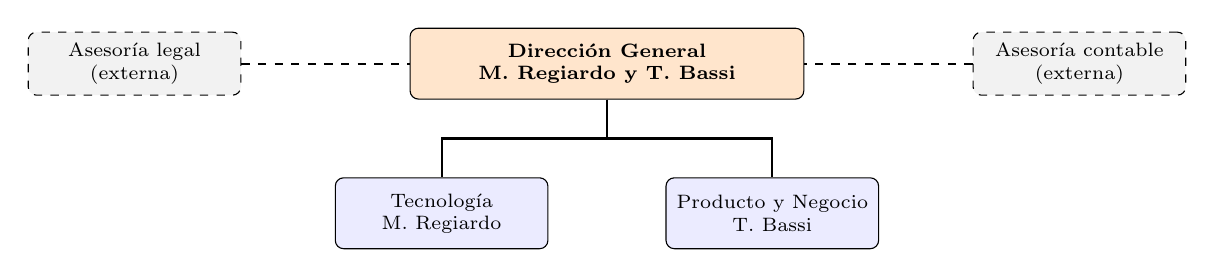
\begin{tikzpicture}[
  area/.style={draw, rounded corners=3pt, align=center, font=\scriptsize, minimum width=2.7cm, minimum height=0.9cm, fill=blue!8},
  dg/.style={draw, rounded corners=3pt, align=center, font=\scriptsize\bfseries, minimum width=5cm, minimum height=0.9cm, fill=orange!20},
  ext/.style={draw, dashed, rounded corners=3pt, align=center, font=\scriptsize, minimum width=2.7cm, minimum height=0.8cm, fill=gray!10},
  lin/.style={thick}]
  \node[dg] (dg) at (0,0) {Dirección General\\ M. Regiardo y T. Bassi};
  \node[area] (tec) at (-2.1,-1.9) {Tecnología\\ M. Regiardo};
  \node[area] (pro) at (2.1,-1.9) {Producto y Negocio\\ T. Bassi};
  \node[ext] (leg) at (-6,0) {Asesoría legal\\ (externa)};
  \node[ext] (con) at (6,0) {Asesoría contable\\ (externa)};
  \draw[lin] (dg) -- ++(0,-0.95) -| (tec);
  \draw[lin] (dg) -- ++(0,-0.95) -| (pro);
  \draw[lin, dashed] (leg) -- (dg);
  \draw[lin, dashed] (con) -- (dg);
\end{tikzpicture}
\caption{organigrama de la etapa de lanzamiento (2 integrantes). Elaboración propia.}
\end{figure}

\subsubsection{Etapa 2: consolidación}
Una vez alcanzado el lanzamiento y validada la propuesta de valor, la estructura se amplía de forma progresiva con profesionales especializados. Se prioriza el fortalecimiento del área tecnológica, con recursos para el desarrollo y el mantenimiento de la plataforma, y la conformación de un área de Marketing y Comunicación que profesionalice la adquisición, la fidelización y el crecimiento de usuarios. Se incorporan también capacidades de administración y finanzas, para mejorar la planificación económica y acompañar el crecimiento de las operaciones comerciales. Los socios fundadores continúan en la Dirección General y supervisan las principales áreas.

\begin{figure}[htbp]
\centering
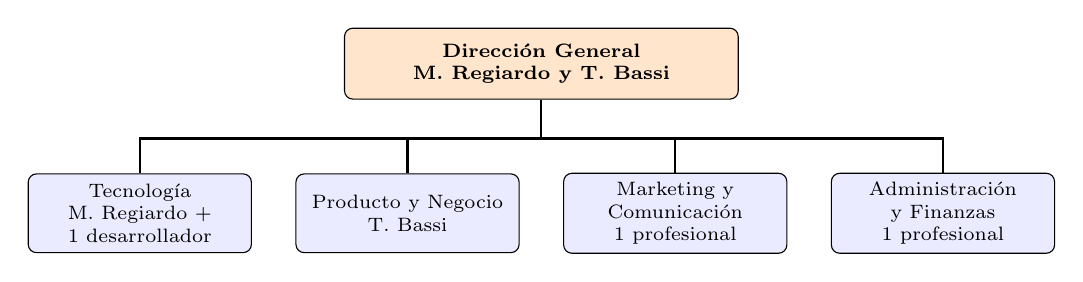
\begin{tikzpicture}[
  area/.style={draw, rounded corners=3pt, align=center, font=\scriptsize, text width=2.6cm, minimum height=1cm, fill=blue!8},
  dg/.style={draw, rounded corners=3pt, align=center, font=\scriptsize\bfseries, minimum width=5cm, minimum height=0.9cm, fill=orange!20},
  lin/.style={thick}]
  \node[dg] (dg) at (0,0) {Dirección General\\ M. Regiardo y T. Bassi};
  \node[area] (tec) at (-5.1,-1.9) {Tecnología\\ M. Regiardo + 1 desarrollador};
  \node[area] (pro) at (-1.7,-1.9) {Producto y Negocio\\ T. Bassi};
  \node[area] (mkt) at (1.7,-1.9) {Marketing y Comunicación\\ 1 profesional};
  \node[area] (adm) at (5.1,-1.9) {Administración y Finanzas\\ 1 profesional};
  \foreach \a in {tec,pro,mkt,adm}{\draw[lin] (dg) -- ++(0,-0.95) -| (\a);}
\end{tikzpicture}
\caption{organigrama de la etapa de consolidación (5 integrantes). Elaboración propia.}
\end{figure}

\subsubsection{Etapa 3: expansión}
En una etapa posterior, asociada al crecimiento de la base de usuarios y a la ampliación del modelo de negocio, la estructura se especializa más. Se fortalecen las áreas existentes con nuevas incorporaciones y se establece un área específica dedicada a la gestión del \textit{marketplace} y de los contenidos digitales, que incluye la vinculación con creadores, la administración del catálogo y el desarrollo de nuevas oportunidades comerciales. Esta evolución acompaña la diversificación de los servicios de \nombreproyecto{} y mantiene una estructura adaptable y orientada al crecimiento sostenible.

\begin{figure}[htbp]
\centering
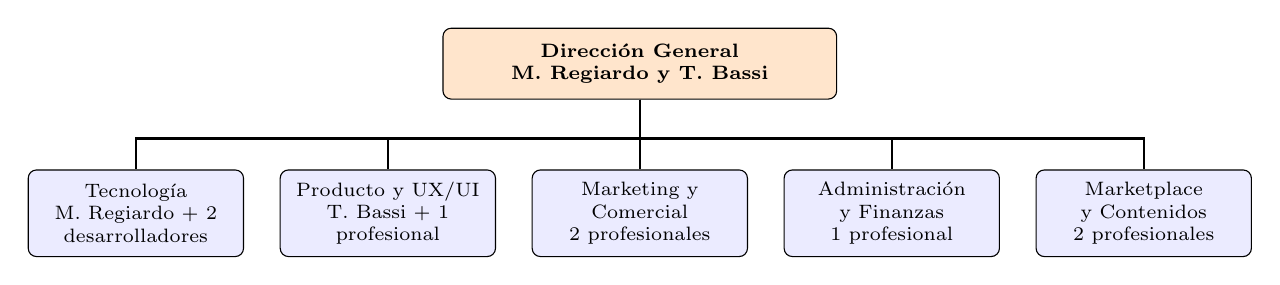
\begin{tikzpicture}[
  area/.style={draw, rounded corners=3pt, align=center, font=\scriptsize, text width=2.5cm, minimum height=1.1cm, fill=blue!8},
  dg/.style={draw, rounded corners=3pt, align=center, font=\scriptsize\bfseries, minimum width=5cm, minimum height=0.9cm, fill=orange!20},
  lin/.style={thick}]
  \node[dg] (dg) at (0,0) {Dirección General\\ M. Regiardo y T. Bassi};
  \node[area] (tec) at (-6.4,-1.9) {Tecnología\\ M. Regiardo + 2 desarrolladores};
  \node[area] (pro) at (-3.2,-1.9) {Producto y UX/UI\\ T. Bassi + 1 profesional};
  \node[area] (mkt) at (0,-1.9) {Marketing y Comercial\\ 2 profesionales};
  \node[area] (adm) at (3.2,-1.9) {Administración y Finanzas\\ 1 profesional};
  \node[area] (mpc) at (6.4,-1.9) {Marketplace y Contenidos\\ 2 profesionales};
  \foreach \a in {tec,pro,mkt,adm,mpc}{\draw[lin] (dg) -- ++(0,-0.95) -| (\a);}
\end{tikzpicture}
\caption{organigrama de la etapa de expansión (10 integrantes). Elaboración propia.}
\end{figure}

La transición entre las etapas no está determinada exclusivamente por plazos temporales, sino principalmente por la evolución de la actividad comercial, el crecimiento de la base de usuarios y las necesidades operativas de la empresa.

\subsection{Filosofía y sistema de trabajo}
La filosofía organizacional de \nombreproyecto{} promueve una cultura de trabajo colaborativa, innovadora y centrada en las necesidades de sus usuarios, en un entorno flexible que favorece la participación de los integrantes, la mejora continua y la adaptación a los cambios tecnológicos y del mercado. Estos valores de la cultura de trabajo complementan los valores nucleares de la organización presentados en la sección~\ref{sec:valores-nucleares}. Los valores que impulsarán a la empresa son:
\begin{itemize}
  \item \textbf{Orientación al usuario y a la comunidad:} las decisiones sobre la evolución del producto se guían por las necesidades de directores de juego y jugadores. Se promueve la participación de la comunidad mediante la recopilación de opiniones, sugerencias y experiencias de uso, para que el desarrollo responda a problemas reales de los usuarios.
  \item \textbf{Innovación y mejora continua:} se fomenta la búsqueda de nuevas soluciones tecnológicas y oportunidades de negocio que mejoren la propuesta de valor. La innovación comprende además la revisión y la optimización de los procesos y funcionalidades existentes.
  \item \textbf{Calidad y confiabilidad:} se prioriza el desarrollo de productos estables, seguros y escalables, con criterios de calidad definidos desde las primeras etapas. Se promueven buenas prácticas de ingeniería de software, documentación, pruebas y mantenimiento que garanticen la sostenibilidad técnica de la plataforma.
  \item \textbf{Colaboración y comunicación:} se mantiene una comunicación abierta entre los integrantes, con intercambio de conocimientos y participación conjunta en la resolución de problemas. Se favorece el trabajo interdisciplinario y la distribución de responsabilidades según las capacidades de cada integrante.
  \item \textbf{Flexibilidad y adaptabilidad:} la organización mantiene una estructura dinámica que responde a las necesidades del negocio y a los cambios del mercado. Se prioriza una gestión eficiente de los recursos, se evitan las estructuras administrativas innecesarias y se incorporan nuevas capacidades de forma progresiva.
\end{itemize}

En términos operativos, el sistema de trabajo se basa en principios de metodologías ágiles, con ciclos iterativos de planificación, desarrollo, evaluación y mejora. Se prioriza la definición de objetivos de corto y mediano plazo, el seguimiento periódico de los avances y la revisión continua de las prioridades.

Asimismo, se promueve el uso de herramientas de colaboración y gestión de proyectos, de procesos de integración y despliegue continuo y de mecanismos de recopilación de retroalimentación de los usuarios. Estas prácticas sostienen la evolución constante del producto, optimizan los tiempos de desarrollo y acompañan el crecimiento de la empresa sin perder flexibilidad organizativa.

\subsection{Requerimientos de recursos humanos}
La planificación de los recursos humanos de \nombreproyecto{} está vinculada con las etapas de crecimiento de la empresa. Se mantiene una estructura de personal reducida durante el lanzamiento y se incorporan progresivamente nuevos profesionales a medida que aumentan las necesidades operativas, comerciales y tecnológicas del emprendimiento. A efectos de la planificación económica se toman como referencia los años 1, 2 y 3 del horizonte para las etapas de lanzamiento, consolidación y expansión, respectivamente. La remuneración de los socios fundadores se difiere hasta alcanzar el punto de equilibrio operativo.

\subsubsection{Etapa 1: lanzamiento}
La plantilla está integrada exclusivamente por los dos socios fundadores, que asumen la dirección general, el desarrollo tecnológico y la gestión del producto y del negocio. No se prevé incorporar personal adicional, pues el volumen inicial de operaciones puede gestionarse con los recursos disponibles. Las necesidades especializadas en materia legal y contable se cubren con profesionales externos.

\subsubsection{Etapa 2: consolidación}
Con el crecimiento de la base de usuarios y la necesidad de fortalecer las actividades comerciales y operativas, se incorporan tres profesionales:
\begin{itemize}
  \item un \textbf{desarrollador de software}, que se integra al área tecnológica para ampliar la capacidad de desarrollo, mantenimiento y evolución de la plataforma;
  \item un profesional de \textbf{Marketing y Comunicación}, orientado a la adquisición y fidelización de usuarios, al posicionamiento de marca y a la gestión de las estrategias de comunicación;
  \item un profesional de \textbf{Administración y Finanzas}, destinado a fortalecer la planificación económica, el control presupuestario y el seguimiento de los indicadores financieros y comerciales.
\end{itemize}
De este modo, los socios fundadores pueden delegar de forma progresiva determinadas actividades operativas y concentrarse en la dirección y en la evolución estratégica del emprendimiento.

\subsubsection{Etapa 3: expansión}
En esta etapa la plantilla crece hasta una estructura aproximada de diez integrantes, con incorporaciones orientadas tanto a fortalecer las áreas existentes como a desarrollar nuevas unidades de negocio:
\begin{itemize}
  \item un \textbf{desarrollador de software adicional}, para ampliar la capacidad técnica y acompañar el crecimiento de la plataforma y sus servicios;
  \item un profesional de \textbf{Producto y Experiencia de Usuario (UX/UI)}, orientado a mejorar la usabilidad, el diseño y la evolución funcional de la plataforma;
  \item un profesional adicional de \textbf{Marketing y Comercial}, especializado en desarrollo de negocios, gestión de comunidades y expansión comercial;
  \item dos profesionales de \textbf{Marketplace y Contenidos}, con conocimientos en gestión de contenidos digitales, vinculación con creadores y administración de catálogos de productos digitales.
\end{itemize}
Estas incorporaciones atienden las nuevas necesidades derivadas de la ampliación del modelo de negocio y de la incorporación del \textit{marketplace}, y preservan la capacidad de adaptación de la estructura.

\subsubsection{Proyección de la plantilla}
La tabla siguiente resume la evolución estimada de los recursos humanos en cada etapa.

\begin{center}
\small
\begin{tabularx}{\textwidth}{|X|c|c|c|}
\hline
\textbf{Área / puesto} & \textbf{Lanzamiento} & \textbf{Consolidación} & \textbf{Expansión}\\ \hline
Dirección General (socios fundadores) & 2 & 2 & 2\\ \hline
Incorporaciones en Tecnología & 0 & 1 & 2\\ \hline
Incorporaciones en Producto y UX/UI & 0 & 0 & 1\\ \hline
Marketing y Comercial & 0 & 1 & 2\\ \hline
Administración y Finanzas & 0 & 1 & 1\\ \hline
Marketplace y Contenidos & 0 & 0 & 2\\ \hline
\textbf{Total de integrantes} & \textbf{2} & \textbf{5} & \textbf{10}\\ \hline
\end{tabularx}
\end{center}

Los dos socios fundadores se contabilizan una única vez, en la fila de Dirección General, aunque desempeñan sus funciones en las áreas de Tecnología y de Producto y Negocio. La dotación total estimada es, por lo tanto, de dos integrantes durante el lanzamiento, cinco durante la consolidación y diez durante la expansión.

Los servicios profesionales externos de asesoramiento legal y contable no se incluyen en estas estimaciones, porque no forman parte de la plantilla permanente de la empresa. Las cantidades son estimaciones de planificación y podrán ajustarse según la evolución de la actividad comercial, la cantidad de usuarios, los ingresos generados y las necesidades operativas que surjan durante el desarrollo del emprendimiento.
